\documentclass[12pt]{article}
\usepackage[russian]{babel}
\usepackage{geometry}

\usepackage{graphicx} % вставка изображений
\usepackage{caption} % описание изображений

%различные цветовые модели
\usepackage[usenames]{color}
\usepackage[dvipsnames,table]{xcolor}
\usepackage{colortbl}

\usepackage{tikz}
\usetikzlibrary{shapes, arrows}
\usepackage{varwidth}
\usepackage{ifthen}

\usepackage{enumitem}

\usepackage{multicol} % вставка изображений в две колонки
\usepackage{makecell} % вставка изображений в две колонки


%циклы foreach в tikz и создание переменных внутри этого окружения
\usepackage{pgffor}
\usepackage{pgfmath}

\usepackage{xifthen}

\usepackage{afterpage}

\usepackage{amssymb}
\usepackage{amsmath}

\usepackage{hyperref}

\usepackage[utf8]{inputenc}

\tikzstyle{connector} = [draw, -latex']
\tikzstyle{line} = [draw, -]
\tikzstyle{dashed} = [draw, -, dash pattern=on 5pt off 5pt]


\usepackage{listings}
\usepackage{listingsutf8}
\usepackage[T2A]{fontenc}
\newcommand{\listingsttfamily}{\usefont{T2A}{PTMono-TLF}{m}{n}}

\lstset{
	language=C,                % choose the language of the code
	numbers=left,                   % where to put the line-numbers
	stepnumber=1,                   % the step between two line-numbers.        
	numbersep=5pt,                  % how far the line-numbers are from the code
	backgroundcolor=\color{black},  % choose the background color. You must add \usepackage{color}
	commentstyle=\color{Gray},
	basicstyle=\listingsttfamily\color{Gray},
	keywordstyle=\color{BurntOrange},
	stringstyle=\color{YellowGreen},
	showspaces=false,               % show spaces adding particular underscores
	showstringspaces=false,         % underline spaces within strings
	showtabs=false,                 % show tabs within strings adding particular underscores
	tabsize=4,                      % sets default tabsize to 2 spaces
	captionpos=b,                   % sets the caption-position to bottom
	breaklines=true,                % sets automatic line breaking
	breakatwhitespace=true,         % sets if automatic breaks should only happen at whitespace
	title=\lstname, 
	inputencoding=utf8,                % show the filename of files included with \lstinputlisting;
	extendedchars=\true,
	keepspaces=true
}

\geometry{top=2cm, bottom=2cm, left=3cm, right=1.5cm}
\textheight=24cm
\textwidth=18cm
\flushbottom 

\oddsidemargin=0pt 
\topmargin=-1.5cm 
\parskip=0.25cm
\parindent=24pt 

\tolerance=2000 

\setcounter{secnumdepth}{0}

\setlist[1]{noitemsep} % sets the itemsep and parsep for all level two lists to 0

\begin{document}
	\begin{center}
		{\parskip=1cm
			МИНИСТЕРСТВО НАУКИ И ВЫСШЕГО ОБРАЗОВАНИЯ РОССИЙСКОЙ ФЕДЕРАЦИИ
			
			ФЕДЕРАЛЬНОЕ ГОСУДАРСТВЕННОЕ БЮДЖЕТНОЕ ОБРАЗОВАТЕЛЬНОЕ УЧРЕЖДЕНИЕ ВЫСШЕГО ОБРАЗОВАНИЯ
			
			{\bf«БЕЛГОРОДСКИЙ ГОСУДАРСТВЕННЫЙ ТЕХНОЛОГИЧЕСКИЙ УНИВЕРСИТЕТ им. В. Г. Шухова»\\(БГТУ им. В. Г. Шухова)}
			
			\begin{figure}[bh]
				\noindent\centering{
					
\includegraphics[width=100mm]{images/start_logo.png}
					\captionsetup{labelformat=empty}
				}
			\end{figure}
			Кафедра программного обеспечения вычислительной техники и автоматизированных систем
		}
		
		{\Large 
			\vspace{1cm}
			{\parskip=0.25cm 
				{\bf Лабораторная работа №4.3}
				
				по дисциплине: «Дискретная математика»
				
				по теме: {\bf Связность}
			}
		}
	\end{center}	
	\begin{flushleft}
		{\leftskip=10cm
			{\vspace{3cm} Выполнил/a: ст. группы ПВ-231}
			
			Чупахина София Александровна
			
			Проверил: Рязанов Юрий Дмитриевич
			
		}
	\end{flushleft}
	\begin{center}
		{\parskip=3cm Белгород, 2024}
	\end{center}
	\newpage

	\tableofcontents
	
	\newpage
	
	\section{Задание 1}
	\label{task1}
	{\bf Текст задания:} Реализовать алгоритм Краскала построения покрывающего леса. 
	
	Поступим как и в прошлой лабораторной работе --- будем представлять граф в формате матрицы смежности, а структуру <<граф>> объявим просто как переименование структуры <<бинарное отношение>>.
	
	Если нам известно количество вершин $n$ и ребер $m$, мы можем точно определить и количество единиц и нулей в матрице смежности. Всего матрица смежности содержит $n^2$ элементов, но поскольку мы работаем с неориентированными графами, можно рассматривать только элементы над главной диагональю: ведь элементы вида $(x, y)$ и $(y, x)$ отражают наличие одного и того же ребра между элементами $x$ и $y$. (Саму главную диагональ мы также не рассматриваем, поскольку элемент не может быть соединен ребром сам с собой, если мы не говорим о псевдографах). Всего в области над главной диагональю $\frac{n^2 - n}{2}$ = $\frac{n\times(n-1)}{2}$ элементов. Действительно, каждый из $n$ элементов может быть соединен ребром с одним из $n-1$ элементов, а чтобы исключить одинаковые пары, мы делим произведение $n\times(n-1)$ на 2. 
	
	Соответственно, если в функцию передается значение --- количество ребер $m$, то в матрице смежности над главной диагональю будет $m$ единиц и $\frac{n\times(n-1)}{2} - m$ нулей. В теле функции создадим граф с пустой матрицей смежности $n\times n$. для Потом запишем ожидаемое количество единиц в переменную ones\_amount, а ожидаемое количество нулей --- в переменную zeros\_amount. Затем, проходя двумя вложенными циклами по элементам над главной диагональю, будем задавать значение каждому из них, сверяясь со значениями этих переменных. Если zeros\_amount равно 0, то значение текущего элемента в матрице смежности может быть равно только 1; если ones\_amount равно 0, то это значение может быть равно только 0; если обе переменные имеют ненулевое значение, то значение элемента определяется значением функции rand() (она возвращает псевдослучайное число, от которого в теле функции потом берется остаток от деления на 2). Текущий элемент матрицы приравнивается к выбранному значению (как и симметричный ему относительно главной диагонали), и в зависимости от того, какое значение было выбрано, уменьшается на 1 переменная zeros\_amount или ones\_amount. Таким образом, за один проход по матрице (вернее, по одной из ее половин) можно сгенерировать случайный граф с заданным количеством вершин и ребер.
	
	Вызвав эту функцию несколько раз для разных значений $n$ и $m$, можем убедиться, что результаты адекватны. 
	
	\lstinputlisting[linerange={1-27, 131-144, 149}]{graphs/graphs_generate_final.c} 
	
	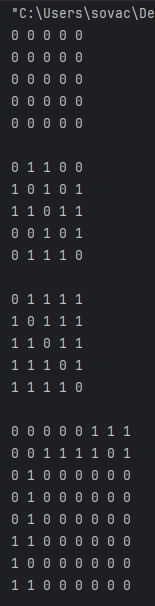
\includegraphics[height=140mm]{images/random_graphs.png}
	
	\section{Задание 2}
	\label{task2}
	
	{\bf Текст задания:} Написать программу, которая:
	
	\begin{description}
	\item[а)] в течение десяти секунд генерирует случайные графы, содержа
	щие $n$ вершин и $m$ ребер; 
	
	\item[б)] для каждого полученного графа определяет, является ли он эй
	леровым или гамильтоновым; 
	
	\item[в)] подсчитывает общее количество сгенерированных графов и ко
	личество графов каждого типа.  
	\end{description}
	
	Результат работы программы представить в виде таблицы (табл. 4). 
	
	Величину $h$ подобрать такой, чтобы в таблице количество строк было в 
	диапазоне от 20 до 30. 
	
	Для выполнения этой задачи нам понадобятся, в первую очередь, функции, определяющие, является ли переданный им граф гамильтоновым или эйлеровым. Для определения того, является ли граф  гамильтоновым, будем методом поиска с возвращением искать в нем хотя бы один гамильтонов цикл. Мы уже пользовались рекурсивным поиском для нахождения маршрутов, цепей и так далее; частично структура программы для определения <<гамильтоновости>> графа будет похожа на структуры ранее написанных программ.
	
	Для выполнения этой задачи нам понадобится три функции. Первая --- вспомогательная функция, проверяющая, включен ли некоторый элемент в последовательность; она понадобится для проверки сложных условий. Вторая --- функция рекурсивного вызова graph\_isHamilton\_, принимабщая на вход непосредственно граф G, формируемый гамильтонов цикл W, индекс формируемой позиции cur\_pos и предварительный результат result. Цепь ее вызовов формирует гамильтонов цикл, а за конкретный вызов задается значение элемента под индексом cur\_pos (отсчет начинается с нуля) в последовательности вершин, отображающей этот цикл. Для этого перебираются все возможные вершины графа, и для каждой проверяется, смежна ли она с последней на текущий момент вершиной в последовательности и не была ли включена в последовательность до сих пор. Если это так, то элемент маршрута под индексом cur\_pos приравнивается к найденному элементу. Затем проверяется, достигла ли последовательность нужной длины (количество вершин в ней на этом этапе должно быть равно количеству вершин в графе в целом). Если это так, то проверяется еще одно условие: соединены ли ребром текущий последний элемент последовательности и элемент, с которого она началась. При выполнении этого второго условия значение result приравнивается к 1. Если выполнено условие о длине, но не выполнено условие о смежности, то никаких действий не предпринимается. Если же условие о длине не выполнено, значит, в последовательность нужно добавлять новые вершины, чтобы она стала (возможно) гамильтоновым циклом. Тогда рекурсивная функция запускается для тех же данных, но с увеличенным на один индексом cur\_pos. После прохода по всем вершинам для данного индекса cur\_pos (и после всех более глубоких рекурсивных вызовов) функция возвращает значение result. И третья функция, graph\_isHamilton --- обертка для рекурсивной функции. Она создает последовательность, которая будет формироваться цепочкой рекурсивных вызовов, задает ее первый элемент (это всегда элемент 1: раз гамильтонов цикл включает в себя все вершины графа, то и вершина 1 будет включена в него, а поскольку это цикл, нет разницы, с какой вершины его начинать) и запускает рекурсивную функцию с cur\_pos равным 1 (нулевой элемент уже сформирован) и предварительным результатом 0.
	
	\lstinputlisting[linerange={28-57}]{graphs/graphs_generate_final.c} 
	
	Однако для определения того, является ли граф эйлеровым, метод поиска с возвращением не пойдет. Ведь в нем длина рассматриваемых последовательностей зависит от  количества ребер, а не вершин, а сами вершины в последовательности могут повторяться. Получается, даже на графе с небольшим количеством вершин при возрастании количества ребер будет увеличиваться длина последовательности, а количество вариантов для рассмотрения будет куда больше, чем для поиска гамильтоновых циклов. Поэтому метод поиска с возвращением применим только для графов с небольшим количеством ребер, и рациональнее применять его тогда, когда нужно получить все эйлеровы циклы. Для проверки же того, является ли граф эйлеровым в принципе, воспользуемся соответствующей теоремой: связный граф является эйлеровым тогда и только тогда, когда все его вершины имеют четную степень.
	
	Для того, чтобы определить степень вершины, достаточно в цикле найти сумму всех элементов соответствующего ей ряда матрицы смежности; степень будет четной, если эта сумма делится нацело на два. Циклом пройдясь по всем вершинам, можно определить, имеют ли они все четную степень. Но как определить связность графа? Если граф связан, значит, из каждой его вершины существует путь в любую другую вершину, неважно какой длины этот путь. Получить матрицу, отображающую, есть ли между вершинами путь заданной блины, можно, возведя матрицу смежности графа в степень, равную этой длине. Но матрица, отображающую, есть ли между вершинами путь в целом --- транзитивное замыкание бинарного отношения, которое задается матрицей смежности графа. Скопируем функцию, возвращающую транзитивное замыкание, из лабораторной работы 3.2. В теле функции graph\_isEuler найдем отношение транзитивного замыкания для матрицы смежности данного графа, а потом будет с помощью цикла проходить по рядам обеих матриц и искать сумму ряда, определяя, таким образом: 1) четна ли степень текущей вершины, 2) все ли элементы отношения транзитивного замыкания равны единице, то есть связан ли каждый элемент исходного графа с каждым. Если для какого-то из рядов хотя бы одно из условий нарушено, значит, граф не является эйлеровым.
	
	\lstinputlisting[linerange={59-83}]{graphs/graphs_generate_final.c} 
	
	Теперь, когда имеются функции, определяющие нужные свойства графа, займемся непосредственно генерацией. Сначала создадим функцию для генерации однородных (с одинаковым количеством и вершин, и ребер) графов и определения их свойств в течение десяти секунд. Перед первой генерацией в теле функции задаются временные метки start и end --- экземпляры структуры timeval из библиотеки <sys.time>. Затем, пока разница между ними не станет больше десяти секунд (эта разница находится с помощью вспомогательной функции), происходит генерация графа с заданным количеством вершин и ребер и определяются его свойства. Если граф эйлеров или гамильтонов, увеличиваются на один значения счетчиков по переданным адресам; вне зависимости от свойств, увеличивается на 1 и счетчик сгенерированных графов в целом. После генерации и определения свойств временная метка end обновляется.
	
	\lstinputlisting[linerange={85-109}]{graphs/graphs_generate_final.c} 
	
	Наконец, последняя функция будет определять шаг, с которым, при заданном количестве вершин графа, будет меняться количество его ребер, и с заданным шагом запускать функцию генерации однородных массивов и выводить на экран значения счетчиков для данного количества вершин и ребер. 
	
	\lstinputlisting[linerange={111-130}]{graphs/graphs_generate_final.c} 
	
	Остается только ввести с клавиатуры значение $n$ и запустить функцию makeTable в теле main.
	
	\lstinputlisting[linerange={132, 146-149}]{graphs/graphs_generate_final.c} 
	
	
	\section{Задание 3}
	\label{task3}

	{\bf Текст задания:} Выполнить программу при $n = 8, 9, 10$ и сделать выводы. 
	
	Запустим программу трижды, вводя с клавиатуры значения 8, 9, 10, и перенесем полученные данные в таблицы ниже.
	
	\begin{tabular}{|m{3cm}|m{3cm}|m{2.5cm}|m{3.5cm}|m{2cm}|}
		\hline
		{\bf Количество вершин} & {\bf Количество ребер} & \multicolumn{3}{|c|}{\bf Количество графов}\\
		\cline{3-5}
		& & {\bf эйлеровых} &{\bf гамильтоновых} & {\bf всех} \\
		\hline
		8 & 8 & 329 & 329 & 2706164 \\
		\hline
		8 & 9 & 296 & 2961 & 2170248 \\
		\hline
		8 & 10 & 5758 & 18781 & 1664216 \\
		\hline
		8 & 11 & 8234 & 70605 & 1331577 \\
		\hline
		8 & 12 & 7380 & 162288 & 994541 \\
		\hline
		8 & 13 & 5763 & 258642 & 845660 \\
		\hline
		8 & 14 & 5488 & 375519 & 753836 \\
		\hline
		8 & 15 & 5333 & 474302 & 725616 \\
		\hline
		8 & 16 & 5074 & 538992 & 716389 \\
		\hline
		8 & 17 & 3936 & 604536 & 732807 \\
		\hline
		8 & 18 & 5724 & 577744 & 679661 \\
		\hline
		8 & 19 & 4064 & 611978 & 692214 \\
		\hline
		8 & 20 & 4922 & 710585 & 776501 \\
		\hline
		8 & 21 & 12396 & 794662 & 853735 \\
		\hline
		8 & 22 & 11960 & 704613 & 750801 \\
		\hline
		8 & 23 & 5070 & 3590176 & 3590176 \\
		\hline
		8 & 24 & 274 & 4484313 & 4484313 \\
		\hline
		8 & 25 & 0 & 4809515 & 4809515 \\
		\hline
		8 & 26 & 0 & 5497014 & 5497014 \\
		\hline
		8 & 27 & 0 & 5546394 & 5546394 \\
		\hline
		8 & 28 & 0 & 6016808 & 6016808 \\
		\hline
	\end{tabular}
	
	\begin{tabular}{|m{3cm}|m{3cm}|m{2.5cm}|m{3.5cm}|m{2cm}|}
		\hline
		{\bf Количество вершин} & {\bf Количество ребер} & \multicolumn{3}{|c|}{\bf Количество графов}\\
		\cline{3-5}
		& & {\bf эйлеровых} &{\bf гамильтоновых} & {\bf всех} \\
		\hline
		9 & 9 & 0 & 0 & 2250347 \\
		\hline
		9 & 10 & 569 & 0 & 1866770 \\
		\hline
		9 & 11 & 494 & 2226 & 1475801 \\
		\hline
		9 & 12 & 2212 & 8453 & 1103489 \\
		\hline
		9 & 13 & 1141 & 26403 & 828961 \\
		\hline
		9 & 14 & 2282 & 56498 & 603688 \\
		\hline
		9 & 15 & 1465 & 100133 & 471878 \\
		\hline
		9 & 16 & 1590 & 144860 & 383106 \\
		\hline
		9 & 17 & 964 & 181004 & 339669 \\
		\hline
		9 & 18 & 1336 & 208463 & 311177 \\
		\hline
		9 & 19 & 781 & 228743 & 300877 \\
		\hline
		9 & 20 & 1129 & 254534 & 306271 \\
		\hline
		9 & 21 & 1141 & 264422 & 303443 \\
		\hline
		9 & 22 & 1188 & 240478 & 270309 \\
		\hline
		9 & 23 & 624 & 221317 & 244116 \\
		\hline
		9 & 24 & 1265 & 213434 & 231075 \\
		\hline
		9 & 25 & 680 & 188389 & 202509 \\
		\hline
		9 & 26 & 505 & 194239 & 205769 \\
		\hline
		9 & 27 & 928 & 240918 & 251222 \\
		\hline
		9 & 28 & 757 & 249320 & 258594 \\
		\hline
		9 & 29 & 709 & 191054 & 197922 \\
		\hline
		9 & 30 & 1299 & 2246412 & 2246412 \\
		\hline
		9 & 31 & 1718 & 3413076 & 3413076 \\
		\hline
		9 & 32 & 17195 & 3860149 & 3860149 \\
		\hline
		9 & 33 & 17632 & 4410086 & 4410086 \\
		\hline
		9 & 34 & 0 & 4357571 & 4357571 \\
		\hline
		9 & 35 & 0 & 4518128 & 4518128 \\
		\hline
		9 & 36 & 3890206 & 3890206 & 3890206 \\
		\hline
	\end{tabular}
	
	\vspace{1.5cm}
	
	\begin{tabular}{|m{3cm}|m{3cm}|m{2.5cm}|m{3.5cm}|m{2cm}|}
		\hline
		{\bf Количество вершин} & {\bf Количество ребер} & \multicolumn{3}{|c|}{\bf Количество графов}\\
		\cline{3-5}
		& & {\bf эйлеровых} &{\bf гамильтоновых} & {\bf всех} \\
		\hline
		10 & 10 & 0 & 0 & 1822419 \\
		\hline
		10 & 11 & 0 & 0 & 1556894 \\
		\hline
		10 & 12 & 0 & 2 & 1256609 \\
		\hline
		10 & 13 & 0 & 947 & 955767 \\
		\hline
		10 & 14 & 625 & 3598 & 732693 \\
		\hline
		10 & 15 & 480 & 8138 & 523783 \\
		\hline
		10 & 16 & 182 & 18236 & 375074 \\
		\hline
		10 & 17 & 351 & 33016 & 272801 \\
		\hline
	\end{tabular}

	\begin{tabular}{|m{3cm}|m{3cm}|m{2.5cm}|m{3.5cm}|m{2cm}|}
	\hline
		10 & 18 & 220 & 47578 & 202974 \\
		\hline
		10 & 19 & 461 & 58483 & 163571 \\
		\hline
		
		10 & 20 & 508 & 78002 & 145503 \\
		\hline
		10 & 21 & 238 & 90230 & 133135 \\
		\hline
		10 & 22 & 114 & 96745 & 126689 \\
		\hline
		10 & 23 & 111 & 101363 & 121978 \\
		\hline
		10 & 24 & 252 & 105400 & 120304 \\
		\hline
		10 & 25 & 239 & 91157 & 102380 \\
		\hline
		10 & 26 & 313 & 92284 & 100954 \\
		\hline
		10 & 27 & 94 & 79453 & 86057 \\
		\hline
		10 & 28 & 103 & 74341 & 79372 \\
		\hline
		10 & 29 & 154 & 66605 & 70394 \\
		\hline
		10 & 30 & 121 & 62977 & 65982 \\
		\hline
		10 & 31 & 123 & 54785 & 57256 \\
		\hline
		10 & 32 & 129 & 52656 & 54679 \\
		\hline
		10 & 33 & 96 & 45336 & 46862 \\
		\hline
		10 & 34 & 87 & 49618 & 50960 \\
		\hline
		10 & 35 & 100 & 55529 & 56756 \\
		\hline
		10 & 36 & 255 & 55409 & 56483 \\
		\hline
		10 & 37 & 228 & 43807 & 44639 \\
		\hline
		10 & 38 & 354 & 1097930 & 1097930 \\
		\hline
		10 & 39 & 0 & 2287160 & 2287160 \\
		\hline
		10 & 40 & 0 & 3026333 & 3026333 \\
		\hline
		10 & 41 & 0 & 3456340 & 3456340 \\
		\hline
		10 & 42 & 0 & 3603233 & 3603233 \\
		\hline
		10 & 43 & 0 & 3978845 & 3978845 \\
		\hline
		10 & 44 & 0 & 3880880 & 3880880 \\
		\hline
		10 & 45 & 0 & 4122492 & 4122492 \\
		\hline
	\end{tabular}
	
	Анализируя данные в таблицах, можем выделить следующие закономерности:
	\begin{itemize}
		\item В большинстве случаев, среди множества случайных графов с одинаковым количеством ребер и вершин эйлеровых графов в несколько десятков раз меньше, чем гамильтоновых,
		\item Нельзя сказать, что количества эйлеровых и гамильтоновых графов изменяются по общему закону; можно найти строки, где количество гамильтоновых графов растет, а эйлеровых --- падает, и наоборот,
		\item Среди графов с равным количеством вершин и ребер существуют и эйлеровы, и гамильтоновы, причем множества эйлеровых и гамильтоновых графов совпадают (это видно на примере, где $n = m = 8$), однако с увеличением числа вершин шансы того, что такие графы будут сгенерированы, сильно падают, потому количество таких графов для $n = 9$ и $n = 10$ в таблице равно 0.
		\item Для ряда случаев, когда количество ребер близится к максимальному, все составленные графы будут гамильтоновыми. В целом с увеличением числа ребер процент гамильтоновых графов среди всех скорее возрастает, тогда как процент эйлеровых графов ведет себя более непредсказуемо.
		\item Для ряда случаев, когда количество ребер близится к максимальному, невозможно составить эйлеров граф; размер этой зоны зависит от того, четно или нечетно количество вершин (для нечетного количества она меньше). От этого же зависит соотношение количества сгенерированных эйлеровых и гамильтоновых графов при максимальном количестве ребер (для полного графа). По сути, когда мы генерируем графы с максимальным количеством ребер, мы все время будем генерировать один и тот же граф; он всегда будет гамильтоновым, поэтому количество сгенерированных в целом и гамильтоновых графов совпадает. Если число вершин нечетно, то полный граф будет эйлеровым, тогда и их количество будет равно общему; если числ овершин четно, то полный граф не является эйлеровым, и число сгененрированных эйлеровых графов будет равно 0.
	\end{itemize}
	
	\section{Задание 4}
	\label{task4}

	{\bf Текст задания:} Привести пример диаграммы графа, который является эйлеровым, но не гамильтоновым. Найти в нем все эйлеровы циклы. 
	
	Зададим следующий граф из пяти вершин и шести ребер.
	
	\begin{tikzpicture}{line width=3pt}
		\def\step{1.75}
		\node[circle, draw=black, minimum height=1cm] at (-\step, 0) (knot1) {1};
		\node[circle, draw=black, minimum height=1cm] at (0, \step) (knot2) {2};
		\node[circle, draw=black, minimum height=1cm] at (\step, 0.5*\step) (knot3) {3};
		\node[circle, draw=black, minimum height=1cm] at (\step, -\step) (knot4) {4};
		\node[circle, draw=black, minimum height=1cm] at (0, -1.5*\step) (knot5) {5};
		
		\path[line, line width = 1.25pt] (knot1) -- (knot2);
		\path[line, line width = 1.25pt] (knot1) -- (knot3);
				
		\path[line, line width = 1.25pt] (knot2) -- (knot3);
		\path[line, line width = 1.25pt] (knot2) -- (knot4);
		\path[line, line width = 1.25pt] (knot2) -- (knot5);
		
		\path[line, line width = 1.25pt] (knot4) -- (knot5);
	\end{tikzpicture}
	
	Вручную пройдя по всем ребрам, мы не сможем найти для него ни одного гамильтонова цикла, но сможем найти как минимум один эйлеров цикл: $[1, 3, 2, 4, 5, 2, 1]$. Но сможем ли мы найти все эйлеровы циклы самостоятельно, а потом доказать, что кроме найденных циклов, других не существует? А сможем ли доказать отсутствие гамильтоновых циклов для этого графа? Чтобы не заниматься этим, напишем программы, выводящие на экран (при их наличии) все эйлеровы и гамильтоновы циклы. Будем использовать для этого уже знакомый нам метод рекурсивного поиска.
	
	Функция graph\_allHamiltonCycles\_, по сути, очень похожа на функцию graph\_isHamilton\_, однако в ней отсутствует аргумент result: вместо того, чтобы приравнивать его к 1, когда подходящая условиям гамильтонова цикла последовательность найдена, последовательность просто выводится на экран с помощью функции printSequence. Обертка этой функции, graph\_allHamiltonCycles, перебирает все возможные элементы, каждый из них назначает на роль первого в созданной последовательности W и для каждого из этих случаев вызывает функцию graph\_isHamilton\_. Так мы получаем все гамильтоновы циклы, а не только начинающиеся с определенной вершины.
	
	\lstinputlisting[linerange={29-59}]{graphs/graphs_cycles_searching.c} 
	
	К рекурсивному поиску эйлеровых циклов будет применяться похожая логика, но при формировании позиции будет проверяться не то, входила ли уже в последовательность такая вершина, а то, входило ли в множество пройденных ребер ребро, образованное рассматриваемой вершиной и предыдущей. После того, как текущая вершина включается в последовательность, в множество пройденных ребер, представленное бинарным отношением, включаются пары, составленные из текущего и предыдущего элемента. Достигла ли последовательность нужной длины, определяется также не количеством вершин графа, а количеством ребер в исходном графе (оно считается с помощью вспомогательной функции). И точно также в качестве первого элемента последовательности в теле функции-обертки поочередно выбираются все вершины графа. 
	
	\lstinputlisting[linerange={61-98}]{graphs/graphs_cycles_searching.c} 
	
	Если мы зададим матрицу смежности этого графа и применим к нему функции graph\_allHamiltonCycles и graph\_allEulerCycles, вывод подтвердит наши догадки: для данного графа не найдено ни одного гамильтонова цикла, но найдено множество эйлеровых.
	
	\lstinputlisting[linerange={19-28, 99-122, 152}]{graphs/graphs_cycles_searching.c} 
	
	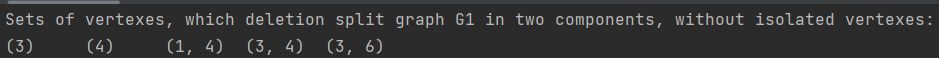
\includegraphics[width=170mm]{images/G1.png}
	
	\section{Задание 5}
	\label{task5}
	
	{\bf Текст задания:}  Привести пример диаграммы графа, который является гамильтоновым, но не эйлеровым. Найти в нем все гамильтоновы циклы. 
	
	Для того, чтобы задать граф, являющийся гамильтоновым, но не эйлеровым, можно задать любую перестановку его вершин и соединить стоящие рядом, а также первую и последнюю вершины, обеспечив наличие в графе хотя бы одного гамильтонова цикла, а потом добавить хотя бы одно ребро, нарушив, таким образом, условие о четности степеней вершин. В графе из пяти вершин зададим перестановку $[1, 3, 4, 2, 5]$, а потом дополнительно проведем ребро между вершинами $4$ и $5$.
	
	\begin{tikzpicture}{line width=3pt}
		\def\step{2}
		\node[circle, draw=black, minimum height=1cm] at (-\step, 0) (knot1) {1};
		\node[circle, draw=black, minimum height=1cm] at (0, \step) (knot2) {2};
		\node[circle, draw=black, minimum height=1cm] at (\step, 0) (knot3) {3};
		\node[circle, draw=black, minimum height=1cm] at (0.5*\step, -1.25*\step) (knot4) {4};
		\node[circle, draw=black, minimum height=1cm] at (-0.5*\step, -1.25*\step) (knot5) {5};
		
		\path[line, line width = 1.25pt] (knot1) -- (knot3);
		\path[line, line width = 1.25pt] (knot1) -- (knot5);
		
		\path[line, line width = 1.25pt] (knot2) -- (knot4);
		\path[line, line width = 1.25pt] (knot2) -- (knot5);
		
		\path[line, line width = 1.25pt] (knot3) -- (knot4);
		\path[line, line width = 1.25pt] (knot4) -- (knot5);
	\end{tikzpicture}
	
	Если мы зададим матрицу смежности этого графа и применим к нему функции graph\_allHamiltonCycles и graph\_allEulerCycles, вывод подтвердит наши догадки: для данного графа не найдено ни одного эйлерова цикла, но найдено несколько гамильтоновых.
	
	\lstinputlisting[linerange={99-100, 114-125, 152}]{graphs/graphs_cycles_searching.c} 
	
	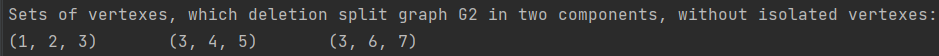
\includegraphics[width=170mm]{images/G2.png}
	
	\section{Задание 6}
	\label{task6}
	
	{\bf Текст задания:} Привести пример диаграммы графа, который является эйлеровым и гамильтоновым. Найти в нем все эйлеровы и гамильтоновы циклы. 
	
	Для того, чтобы задать граф, являющийся и гамильтоновым, и эйлеровым, можно задать любую перестановку его вершин и соединить стоящие рядом, а также первую и последнюю вершины, обеспечив наличие в графе хотя бы одного гамильтонова цикла. Если не добавлять в граф ни одного ребра после этого, то полученный гамильтонов цикл будет проходить по всем ребрам графа, а значит, будет являться также и эйлеровым. В графе из пяти вершин зададим перестановку $[1, 2, 3, 4, 5]$ и соединим соответствующие вершины.
		
	\begin{tikzpicture}{line width=3pt}
		\def\step{2}
		\node[circle, draw=black, minimum height=1cm] at (-\step, 0) (knot1) {1};
		\node[circle, draw=black, minimum height=1cm] at (0, \step) (knot2) {2};
		\node[circle, draw=black, minimum height=1cm] at (\step, 0) (knot3) {3};
		\node[circle, draw=black, minimum height=1cm] at (0.5*\step, -1.25*\step) (knot4) {4};
		\node[circle, draw=black, minimum height=1cm] at (-0.5*\step, -1.25*\step) (knot5) {5};
		
		\path[line, line width = 1.25pt] (knot1) -- (knot2);
		\path[line, line width = 1.25pt] (knot1) -- (knot5);
		\path[line, line width = 1.25pt] (knot2) -- (knot3);
		\path[line, line width = 1.25pt] (knot3) -- (knot4);
		\path[line, line width = 1.25pt] (knot4) -- (knot5);
	\end{tikzpicture}
	
	Если мы зададим матрицу смежности этого графа и применим к нему функции graph\_allHamiltonCycles и graph\_allEulerCycles, вывод подтвердит наши догадки: для данного графа существуют как эйлеровы, так и гамильтоновы циклы.
	
	\lstinputlisting[linerange={99-100, 127-138, 152}]{graphs/graphs_cycles_searching.c} 
	
	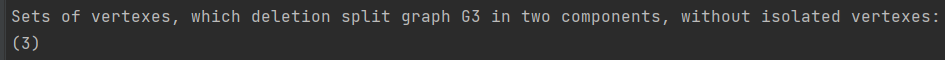
\includegraphics[width=170mm]{images/G3.png}
	
	\section{Задание 7}
	\label{task7}
	
	{\bf Текст задания:} Привести пример диаграммы графа, который не является ни эйлеровым, ни гамильтоновым.
	
	Для того, чтобы задать граф, не являющийся ни гамильтоновым, ни эйлеровым, можно расположить ребра между вершинами графа таким образом, чтобы существовала вершина, смежная только с одной вершиной. Тогда при формировании маршрута, при прохождении через эту вершину, продвинуться дальше не будет возможности, не пройдя еще раз по тому единственному ребру, которое вело к единственной смежной с ней вершине. Значит, будет нарушено условие и эйлерова, и гамильтонова цикла. В графе из пяти вершин  проведем ребра так, чтобы вершины $1$ и $5$ имели только одну смежную вершину. 
	
	\begin{tikzpicture}{line width=3pt}
		\def\step{2}
		\node[circle, draw=black, minimum height=1cm] at (-\step, 0) (knot1) {1};
		\node[circle, draw=black, minimum height=1cm] at (0, \step) (knot2) {2};
		\node[circle, draw=black, minimum height=1cm] at (\step, 0) (knot3) {3};
		\node[circle, draw=black, minimum height=1cm] at (0.5*\step, -1.25*\step) (knot4) {4};
		\node[circle, draw=black, minimum height=1cm] at (-0.5*\step, -1.25*\step) (knot5) {5};
		
		\path[line, line width = 1.25pt] (knot1) -- (knot2);
		\path[line, line width = 1.25pt] (knot2) -- (knot3);
		\path[line, line width = 1.25pt] (knot2) -- (knot4);
		\path[line, line width = 1.25pt] (knot2) -- (knot5);
		\path[line, line width = 1.25pt] (knot3) -- (knot4);
	\end{tikzpicture}
	
	Если мы зададим матрицу смежности этого графа и применим к нему функции graph\_allHamiltonCycles и graph\_allEulerCycles, вывод подтвердит наши догадки: для данного графа не найдено ни одного эйлерова, равно как и ни одного гамильтонова цикла.
	
	\lstinputlisting[linerange={99-100, 140-152}]{graphs/graphs_cycles_searching.c} 
	
	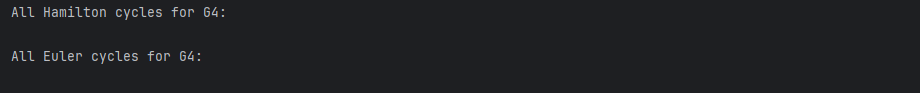
\includegraphics[width=170mm]{images/G4.png}
	
	\section{Вывод}
	\label{final}
	
	Среди маршрутов --- последовательностей инцидентных ребер и вершин в графе, которые чаще расматриваются как последовательности смежных вершин --- можно выделить отдельный класс: циклы. Дополнительные свойства маршрутов позволяют выделять среди них цепи, простые цепи, циклы и простые циклы. У циклов можно выделять разные свойства: например, свойство простоты --- цикл называется простым, если ни одна из вершин в нем, кроме первой и последней, не повторяется. В данной же работе обосый интерес для нас представляли понятия гамильтонова и эйлерова цикла. Гамильтоновым циклом называется простой цикл, куда входят все вершины графа. Эйлеровым циклом называется цикл, в котором могут повторяться вершины, но в который входят без повторений все ребра графа. Если в графе существует хотя бы один гамильтонов или эйлеров цикл, он называется соотвественно гамильтоновым или эйлеровым.
	
	В ходе лабораторной работы написали ряд функций, которые как определяют, является ли граф гамильтоновым или эйлеровым, так и находят в нем все гамильтоновы и эйлеровы циклы; путем генерации большого числа графов определили, как много гамильтоновых и эйлеровых графов содержится среди графов с тем или иным количеством ребер и вершин; привели примеры графов, которые обладают только одним из этих свойств, двумя свойствами сразу или ни одним из них; применили эти функции, чтобы найти все гамильтоновы и эйлеровы циклы в составленных графах.

\end{document}